\documentclass{if-beamer}

% --------------------------------------------------- %
%                  Presentation info	              %
% --------------------------------------------------- %
\title[Lecture 8]{Lecture 8}
\subtitle{Arrays And Dynamic Allocation Using Pointers}
\author{Instructor: Ashley Gannon}
\date{ISC3313 Fall 2021}
\logo{

\includegraphics[scale=0.08]{figures/FSULogo.png}
}
\subject{Presentation subject}

% --------------------------------------------------- %
%                    Title + Schedule                 %
% --------------------------------------------------- %
\begin{document}

\begin{frame}
  \titlepage  
\end{frame}
% --------------------------------------------------- %
%                      Presentation                   %
% --------------------------------------------------- %
\section{Warm Up Activity}
\begin{frame}
\frametitle{Activity}
Using slide 24 from the last lecture \textit{NamespacesVariableScopesControlStructuresFunctions}, write a function \texttt{division} that 
\begin{itemize}
	\item takes in two arguments,\\
	\item divides them,\\
	\item and returns a number.\\
\end{itemize}   
\vspace{10pt}
Post your code in the discussion board \textbf{Division function} for participation credit. Your code doesn't have to be working, or even correct- \textbf{just make an honest effort}!  
\end{frame}

\section{Arrays}

\begin{frame}
\frametitle{Arrays}
\vspace{1.5cm}
Up until now we have used variables to represent a single quantity.
What if there are many quantities?  An array is simply a means to store
multiple values, to be accessed by a single variable name. The syntax
is \\
\vspace{5pt}
{\texttt{{type arrayname[dimension]}}} \\
\vspace{5pt}
An example is: \\
\vspace{5pt}
\texttt{int myarr[4];} \\
\texttt{myarr[0] = 4;} \\
\texttt{myarr[1] = 1;} \\
\texttt{myarr[2] = 8;} \\
\texttt{myarr[3] = 13;} \\
\end{frame}

\begin{frame}
\frametitle{Arrays}
Arrays can also be initialized as \\
\vspace{5pt}
\texttt{int myarr[4] = \{4, 1, 8, 13\}} \\
\vspace{5pt}
The size of the array does not need to be specified if it is
initialized this way. The compiler will figure it out. The alternative
declaration is: \\
\vspace{5pt}
\texttt{int myarr[] = \{4, 1, 8, 13\}}
\end{frame}


\begin{frame}
\frametitle{Indexing}
We access the elements of an array using the index, which is the value
that goes in the square brackets. The index must be an integer. We
could also use a \texttt{for} loop to fill in the values: \\[0.5cm]
\vspace{5pt}
\texttt{int myarr[4];}\\
\texttt{for (int i = 0; i < 4; i++)}\\
\texttt{\{}\\
\qquad \texttt{cin >> myarr[i];}\\
\texttt{\}}\\
\vspace{10pt}
Here the variable \texttt{i} is the index.
\end{frame}

\begin{frame}
\frametitle{Addresses in memory}
Consider the array: \\
\vspace{5pt}
\texttt{\{78, 45, 12, 89, 56\}} \\
\vspace{5pt}
The elements of this array are stored in contiguous memory addresses.  In
this figure, the address increases by 2 due to the size of each integer
element (2 bytes, 1 address space per byte).
\begin{figure}
\center
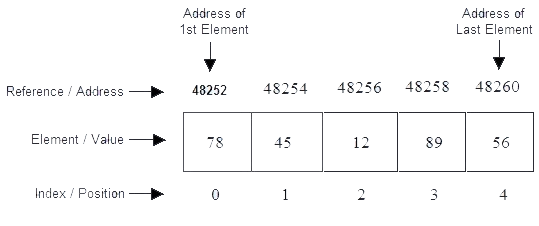
\includegraphics[width=0.8\textwidth]{figures/array.png}
\end{figure}
\end{frame}

\begin{frame}
\frametitle{Character arrays}
One simple application of arrays is a string. A string is an array of
type \texttt{char}. We could create a string as follows: \\
\vspace{5pt}
\texttt{char mystring[20] = \{'H','E','L','L','O','\textbackslash 0' \}; } \\
\vspace{5pt}
Notice that at the end we make use of the null character \texttt{'\textbackslash 0'}, which specifies the end of a character array. We could also use
\vspace{5pt}
\texttt{char mystring[20] = "Hello";} \\
\vspace{5pt}
This is a string literal and always has a null character (done automatically)
\end{frame}

\begin{frame}
\frametitle{Out of bounds indexing}
\begin{itemize}
\item<1-> \texttt{C++} does not perform array bounds checking for you
\item<2-> This means that you may try to access an element which is outside of the array's bounds
\item<3-> This is an example of a runtime error, and it will likely cause the program
to crash
\item<4-> Even worse, it may \textit{not} crash but instead
overwrite other data in your program
\end{itemize}
\end{frame}

\begin{frame}
\frametitle{Class activity}
Write a program that asks the user to enter an 8-digit password.Your program should:\\

\begin{itemize}
	\item Allow the user to type the password
	\item Store it in a \texttt{char} array
	\item Print the password back to the user
\end{itemize}
You should manually put the null character at the end of the array after the password is entered so that you can print the array with \texttt{cout}.

\vspace{10pt}
Post your code in the discussion board \textbf{Password Code} for participation credit. 
\end{frame}

\section{Dynamic allocation with pointers}

\begin{frame}
\frametitle{Static versus dynamic allocation}
So far we have seen static arrays.
\begin{itemize}
\item Their size must be known (specified by you) at compile-time
\item Their size cannot be determined once the program begins executing
\end{itemize}

The size of a dynamic array can be determined at run-time. These are
far more useful. However, they require knowledge of \textit{pointers}!
\end{frame}

\begin{frame}
\frametitle{Pointers}
Pointers are a type of variable whose value is actually a memory
address (of another variable). We saw how to get the address of a
variable using referencing. Recall the example: \\
\vspace{5pt}
\texttt{int b = 5;} \\
\texttt{int\&c = b;} \\
\texttt{b = 3;} \\
\texttt{cout << c << endl;} \\
\vspace{5pt}
There is a difference between using \texttt{\&} in the declaration
(left of equal sign) and with the variable itself (right of equal sign).
\end{frame}

\begin{frame}
\frametitle{Address-of operator}
If we use the \texttt{\&} symbol next to the variable, it acts as an
'address-of' operator: \\
\vspace{5pt}
\texttt{int a = 5;} \\
\texttt{cout << \&a << endl;} \\
\vspace{5pt}
This would just print the address given for \texttt{a} in memory. Not exactly useful, yet.
\end{frame}

\begin{frame}
\frametitle{Pointers and address-of}
The pointer is used to store the address of a variable. We can declare
a pointer using \texttt{\textasteriskcentered} as follows: \\
\vspace{5pt}
\texttt{int* p;} \\
\vspace{5pt}
Then we can set it to the \textit{address} of any variable:\\
\vspace{5pt}
\texttt{int a = 5;}\\
\texttt{p = \&a;}\\
\end{frame}

\begin{frame}
\frametitle{Dereferencing}
Dereferencing is how you find out what \textit{value} is at the
\textit{address} pointed to by a pointer. We again make use of the
\texttt{\textasteriskcentered} symbol, but again, it has a different
meaning then in a declaration. Consider the following code:\\
\vspace{5pt}
\texttt{int a = 5;}\\
\texttt{int* p = \&a;}\\
\texttt{cout << *p << endl;}\\
\end{frame}

\begin{frame}
\frametitle{Dereferencing}
We can also use dereferencing to \textit{change} the value at the
address pointed to by the pointer. consider the same example as before:\\
\vspace{5pt}
\texttt{int a = 5;}\\
\texttt{int* p = \&a;}\\
\texttt{*p = 3;}\\
\texttt{cout << a << endl;}\\
\end{frame}

\begin{frame}
\frametitle{\LARGE Dynamic arrays with pointers}
Pointers are very useful when working with arrays. To create an array
with a variable size we would do the following: \\
\vspace{5pt}
\texttt{int n = 10;}\\
\texttt{int* p = new int[n];}\\
\vspace{5pt}
The \texttt{new} operator is another special keyword that allocates
\textit{memory} for an array of integers. Not the same thing as a
static array. YOU are responsible for this memory!
\begin{figure}
\center
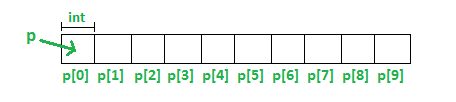
\includegraphics[width=0.7\textwidth]{figures/pointerarray.png}
\end{figure}
\end{frame}

\begin{frame}
\frametitle{\LARGE Dynamic arrays with pointers}
\vspace{1.2cm}
Once you create this memory you can access it using the same syntax as a static array:\\
\vspace{5pt}
\texttt{int n = 10;}\\
\texttt{int* p = new int[n];}\\
\texttt{for (int i = 0; i < 10; i++)}\\
\texttt{\{}
\texttt{p[i] = i;}\\
\texttt{\}}
\texttt{cout << p[5] << endl;}\\
\vspace{5pt}
Note that if you do \texttt{\textasteriskcentered p} now, it is the
value of the first entry (\texttt{p[0]}). The pointer always points to
the first element in memory.
\end{frame}

\end{document}
